\section{Periodic Hurwitz correlations and the gamma ladder}
\label{gamma:sec:correlations}

The polynomial moments in the repository describe one way to pair a
Hurwitz jet with a test function. A second useful pairing is translation
on the circle. It keeps the complete shift variable and produces
polylogarithms, rather than only their values at unity. Its most useful
consequence below is an exact convergent expansion proving strict
convexity of the periodic autocorrelation of $\log\Gamma$.

The underlying Fourier calculation is classical. In particular, the
zero-shift product integral is Theorem~3.1 of Espinosa--Moll
\cite{gamma:EspinosaMoll2002}; their Example~7.2 gives the familiar square
moment of $\log\Gamma$. The Fourier transform of Hurwitz zeta, Lerch's
identity, and the local polylogarithm expansion are classical formulas
\cite{gamma:DLMF}. The circle interpretation also belongs to the
spectral framework discussed by Gay--Sebbar \cite{gamma:GaySebbar2024}.
We present the shifted calculus with its precise domains, derive a
uniform family of Stieltjes-primitive cusp polynomials, and prove the
convexity result. These are extensions developed here, without a claim
of exhaustive bibliographic priority.

For $0<x<1$, let $\mathcal Z_s(x)=\zeta(s,x)$ and extend this function
periodically, with its values at integers immaterial in integrals.
Write $\{x\}=x-\lfloor x\rfloor$. For $0<a<1$ set
\begin{equation}
 C(s,t;a)=\int_0^1\zeta(s,x)\zeta(t,\{x+a\})\,dx.
 \label{gamma:eq:C-definition}
\end{equation}
The two singularities occur at distinct points, $x=0$ and $x=1-a$.

\begin{theorem}[Shifted Hurwitz product]
\label{gamma:thm:shifted-product}
For $0<a<1$, the integral \eqref{gamma:eq:C-definition} converges
absolutely and is jointly holomorphic on
$\Re s<1$, $\Re t<1$. On this domain,
\begin{align}
 C(s,t;a)
 ={}&\frac{\Gamma(1-s)\Gamma(1-t)}{(2\pi)^{2-s-t}}
 \biggl[
 e^{\pi i(t-s)/2}\Li_{2-s-t}(e^{2\pi ia})\notag\\
 &\hspace{44mm}
 +e^{\pi i(s-t)/2}\Li_{2-s-t}(e^{-2\pi ia})
 \biggr].
 \label{gamma:eq:shifted-product}
\end{align}
At $a=0$, the same formula with both polylogarithms replaced by
$\zeta(2-s-t)$ holds on the absolute-convergence domain
\begin{equation}
 \Re s<1,\qquad \Re t<1,\qquad \Re(s+t)<1.
 \label{gamma:eq:zero-shift-domain}
\end{equation}
All spectral derivatives can be taken under the integral on compact
subsets of these domains.
\end{theorem}

\begin{proof}
The shift identity gives
$\zeta(s,x)=x^{-s}+\zeta(s,1+x)$.
On every compact subset of $\Re s<1$, this and its spectral derivatives
are bounded near zero by a constant times
$x^{-\sigma}(1+|\log x|^r)+1$, with some $\sigma<1$.
For a nonzero shift, the two endpoint singularities are separated.
These bounds give absolute convergence, local domination, and joint
holomorphy. At zero shift the extra condition in
\eqref{gamma:eq:zero-shift-domain} controls the product $x^{-s-t}$.

For $\Re s<0$ the classical Hurwitz Fourier series is absolutely
convergent:
\begin{equation}
 \mathcal Z_s(x)=\Gamma(1-s)
       \sum_{n\ne0}(2\pi in)^{s-1}e^{2\pi inx},
 \qquad \log(2\pi in)=\log(2\pi|n|)+\tfrac{\pi i}{2}\operatorname{sgn}n.
 \label{gamma:eq:hurwitz-fourier}
\end{equation}
Multiplying the two series and integrating leaves the terms with
opposite Fourier indices. Splitting the result into positive and
negative indices proves \eqref{gamma:eq:shifted-product} when
$\Re s,\Re t<0$. The right side is holomorphic on the larger product
of half-planes: the order dependence of $\Li_w(z)$ is entire for fixed
$z=e^{\pm2\pi ia}\ne1$, and the gamma factors have no poles there.
Holomorphic continuation proves the assertion. The zero-shift proof
uses the same argument on the connected domain
\eqref{gamma:eq:zero-shift-domain}.
\end{proof}

The domain distinction matters: a nonzero shift permits $\Re s$ and
$\Re t$ arbitrarily close to $1$ individually, whereas coincident
singularities impose an additional sum condition.

\subsection{A factorization through one Hurwitz order}

Put $u=s+t$ and define the holomorphic germ
\begin{equation}
 F(s,t)=\frac{\Gamma(1-s)\Gamma(1-t)}{\Gamma(2-s-t)}
 \frac{\cos\bigl(\pi(s-t)/2\bigr)}{\cos\bigl(\pi(s+t)/2\bigr)}.
 \label{gamma:eq:F}
\end{equation}
For example, $F$ is holomorphic when $|s|+|t|<1$, and $F(0,0)=1$.
Let
$C^+(s,t;a)=\tfrac12[C(s,t;a)+C(t,s;a)]$.

\begin{proposition}[Symmetric factorization]
\label{gamma:prop:factorization}
In a neighborhood of $(s,t)=(0,0)$, for $0<a<1$,
\begin{align}
 C^+(s,t;a)
 &=-\frac{F(s,t)}2\bigl[\zeta(u-1,a)+\zeta(u-1,1-a)\bigr],
 \label{gamma:eq:factorization}\\
 C(s,t;0)&=-F(s,t)\zeta(u-1).
 \label{gamma:eq:factorization-zero}
\end{align}
\end{proposition}

\begin{proof}
Symmetrizing \eqref{gamma:eq:shifted-product} produces
\[
 \frac{\Gamma(1-s)\Gamma(1-t)}{(2\pi)^{2-u}}
 \cos\frac{\pi(s-t)}2
 \bigl[\Li_{2-u}(e^{2\pi ia})+\Li_{2-u}(e^{-2\pi ia})\bigr].
\]
Apply the even part of \eqref{gamma:eq:hurwitz-fourier} at order $u-1$:
\[
 \zeta(u-1,a)+\zeta(u-1,1-a)
 =-\frac{2\Gamma(2-u)\cos(\pi u/2)}{(2\pi)^{2-u}}
 \bigl[\Li_{2-u}(e^{2\pi ia})+\Li_{2-u}(e^{-2\pi ia})\bigr].
\]
This proves the first formula. Letting $a\downarrow0$ proves the second.
The zero-shift formula is also exactly the beta-function form of the
classical Espinosa--Moll product integral.
\end{proof}

\subsection{All spectral jets and Stieltjes antiderivatives}

For $r\ge0$, define
\begin{equation}
 J_r(x)=\left.\partial_s^r\zeta(s,x)\right|_{s=0}.
 \label{gamma:eq:J}
\end{equation}
Then $J_0(x)=\tfrac12-x$ and
$J_1(x)=\log\Gamma(x)-\tfrac12\log(2\pi)$.
All $J_r$ belong to $L^p(0,1)$ for every finite $p$, since
\begin{equation}
 J_r(x)=(-\log x)^r+\zeta^{(r)}(0)+O(x)
 \qquad(x\downarrow0).
 \label{gamma:eq:J-endpoint}
\end{equation}
Their means vanish: differentiate
$\int_0^1\zeta(s,x)\,dx=0$ near $s=0$.

The Stieltjes convention is
$\zeta(1+v,x)=v^{-1}+\sum_{n\ge0}(-1)^n\gamma_n(x)v^n/n!$.
The classical argument-derivative identity gives
\begin{equation}
 J_{n+1}'(x)=(-1)^{n+1}(n+1)\gamma_n(x),\qquad
 \mathcal G_n(x):=\int_1^x\gamma_n(y)\,dy
 =\frac{(-1)^{n+1}}{n+1}
       [J_{n+1}(x)-\zeta^{(n+1)}(0)].
 \label{gamma:eq:stieltjes-primitives}
\end{equation}
Thus all correlations of these antiderivatives are mixed spectral
derivatives of \eqref{gamma:eq:shifted-product} at $s=t=0$.
This identifies their polylogarithm order derivatives without numerical
integer-relation searches.

\begin{theorem}[Universal cusp polynomials and a convergent expansion]
\label{gamma:thm:jet-cusp}
For nonnegative integers $r,m$, let
\begin{equation}
 E_{r,m}(a)=\int_0^1[J_r(\{x+a\})-J_r(x)]
                       [J_m(\{x+a\})-J_m(x)]\,dx.
 \label{gamma:eq:mixed-increments}
\end{equation}
For $0<a<1$, with $L_a=\log(1/a)$,
\begin{align}
 E_{r,m}(a)
 ={}&aP_{r,m}(L_a)\notag\\
 &+2\sum_{j\ge1}\frac{a^{2j}}{(2j)!}
 \left.\partial_s^r\partial_t^m
 \left[F(s,t)(u-1)_{2j}\zeta(u+2j-1)\right]\right|_{s=t=0},
 \label{gamma:eq:all-jet-expansion}
\end{align}
where $(z)_n=z(z+1)\cdots(z+n-1)$ and
\begin{equation}
 P_{r,m}(L)=
 \left.\partial_s^r\partial_t^m
              [F(s,t)e^{L(s+t)}]\right|_{s=t=0}.
 \label{gamma:eq:cusp-polynomial}
\end{equation}
The series converges locally uniformly for $0<a<1$. Each
$P_{r,m}$ is a monic polynomial of degree $r+m$, and
$E_{r,m}(a)=aP_{r,m}(L_a)+O(a^2)$ as $a\downarrow0$.
The apparent pole in the $j=1$ coefficient is removable.
\end{theorem}

\begin{proof}
Translation invariance and exchange of the two indices give
\[
 E_{r,m}(a)=
 2\left.\partial_s^r\partial_t^m
     [C(s,t;0)-C^+(s,t;a)]\right|_{s=t=0}.
\]
Use \eqref{gamma:eq:factorization}--\eqref{gamma:eq:factorization-zero},
then the shift identity and the Taylor series at Hurwitz parameter $1$:
\begin{align*}
 &\zeta(u-1,a)+\zeta(u-1,1-a)-2\zeta(u-1)\\
 &\qquad=a^{1-u}
     +2\sum_{j\ge1}\frac{(u-1)_{2j}}{(2j)!}
                         \zeta(u+2j-1)a^{2j}.
\end{align*}
The Taylor radius is $1$, the distance from parameter $1$ to its
nearest singularity $0$. This proves convergence and permits spectral
differentiation on smaller compact sets. At $j=1$,
$(u-1)_2=u(u-1)$ cancels the pole of $\zeta(1+u)$.
The singular term is $aF(s,t)e^{L_a(s+t)}$, giving
\eqref{gamma:eq:cusp-polynomial}. Its leading coefficient is
$F(0,0)=1$. The remaining series starts at $a^2$.
\end{proof}

All coefficients in the cusp polynomials are explicit. A convenient
closed generating formula is
\begin{align}
 \log F(s,t)={}&-\log(1-s-t)
   +\sum_{n\ge2}\frac{\zeta(n)}n
       [s^n+t^n-(s+t)^n]\notag\\
 &+\sum_{\substack{n\ge2\\n\ {
m even}}}
       \frac{2(1-2^{-n})\zeta(n)}n
       [(s+t)^n-(s-t)^n].
 \label{gamma:eq:log-F}
\end{align}
It follows from the gamma and cosine products and converges near zero.
For instance,
\begin{align}
 P_{1,1}(L)&=L^2+2L+2+\frac{\pi^2}{3},
 \label{gamma:eq:P11}\\
 P_{1,2}(L)&=L^3+3L^2+\left(6+\frac{2\pi^2}{3}\right)L
               +6+\frac{2\pi^2}{3}-2\zeta(3),
 \label{gamma:eq:P12}\\
 P_{2,2}(L)&=L^4+4L^3+\left(12+\frac{4\pi^2}{3}\right)L^2
       +\left(24+\frac{8\pi^2}{3}-8\zeta(3)\right)L\notag\\
 &\qquad+24+\frac{8\pi^2}{3}-8\zeta(3)+\frac{7\pi^4}{45}.
 \label{gamma:eq:P22}
\end{align}
In particular the first nontrivial Stieltjes primitive satisfies
\[
 \int_0^1[\mathcal G_1(\{x+a\})-\mathcal G_1(x)]^2\,dx
   =\frac a4P_{2,2}(\log(1/a))+O(a^2).
\]
The exact higher coefficients in \eqref{gamma:eq:all-jet-expansion}
involve Stieltjes constants at the $j=1$ resonance and zeta jets at
positive odd integers for $j\ge2$.

\section{Strict convexity of the periodic log-gamma correlation}
\label{gamma:sec:convexity}

Write
\[
 g(x)=\log\Gamma(x),\qquad \ell=\log(2\pi),\qquad A=\gamma+\ell,
\]
\[
 R(a)=\int_0^1g(x)g(\{x+a\})\,dx,\qquad
 S(a)=\int_0^1[g(\{x+a\})-g(x)]^2\,dx.
\]
Both extend continuously to the circle, and
$S(a)=2[R(0)-R(a)]$ and $S(1-a)=S(a)$.
Here the square in $S$ is an ordinary square of real-valued functions.

\begin{proposition}[Two exact evaluations of the correlation]
\label{gamma:prop:loggamma-correlation}
For $0<a<1$, set $B_2(a)=a^2-a+1/6$ and write
$\Li_w^{[j]}(z)=\partial_w^j\Li_w(z)$ for spectral derivatives.
Then
\begin{align}
 R(a)={}&\frac{\ell^2}{4}
 +\frac1{2\pi^2}\Re\left[
     \Li_2^{[2]}(e^{2\pi ia})-2A\Li_2^{[1]}(e^{2\pi ia})
     +\left(A^2+\frac{\pi^2}{4}\right)\Li_2(e^{2\pi ia})\right]
 \label{gamma:eq:R-polylog}\\
 ={}&\frac{\ell^2}{4}
    -\frac{\zeta''(-1,a)+\zeta''(-1,1-a)}2
    -\zeta'(-1,a)-\zeta'(-1,1-a)
    +\left(1+\frac{\pi^2}{6}\right)B_2(a).
 \label{gamma:eq:R-hurwitz}
\end{align}
\end{proposition}

\begin{proof}
Since $g=J_1+\ell/2$ and $\int J_1=0$, the desired centered correlation
is $\partial_s\partial_t C(s,t;a)|_{0,0}$.
Apply these derivatives to \eqref{gamma:eq:shifted-product}.
The mixed derivative of the phase contributes $\pi^2/4$, giving
\eqref{gamma:eq:R-polylog}.
For \eqref{gamma:eq:R-hurwitz}, use the symmetric factorization,
$F_s(0,0)=F_t(0,0)=1$, $F_{st}(0,0)=2+\pi^2/3$, and
$\zeta(-1,a)+\zeta(-1,1-a)=-B_2(a)$.
\end{proof}

\begin{theorem}[Convergent odd-zeta expansion and strict concavity]
\label{gamma:thm:loggamma-concavity}
For every $0<a<1$,
\begin{align}
 S(a)={}&a\left[\log^2\frac1a+2\log\frac1a+2+\frac{\pi^2}{3}\right]
       +\left(2\gamma_1-\frac{\pi^2}{3}\right)a^2\notag\\
 &-\sum_{j=2}^{\infty}\frac{2a^{2j}}{j(2j-1)}
       \left[H_{2j-2}\zeta(2j-1)+\zeta'(2j-1)\right].
 \label{gamma:eq:loggamma-increment-series}
\end{align}
This is a convergent identity, not only an asymptotic expansion.
Every bracket in the series is strictly positive. The function $S$ is
strictly concave on $(0,1)$, so $R$ is strictly convex there. Consequently
$S$ has a unique maximum, and $R$ a unique minimum, at $a=1/2$.
\end{theorem}

\begin{proof}
Specialize Theorem~\ref{gamma:thm:jet-cusp} to $r=m=1$.
For the quadratic term,
\[
 u(u-1)\zeta(1+u)
   =-1+(1-\gamma)u+(\gamma+\gamma_1)u^2+O(u^3).
\]
Its product with $F(s,t)$ has mixed derivative
$-(2+\pi^2/3)+2(1-\gamma)+2(\gamma+\gamma_1)
=2\gamma_1-\pi^2/3$.
For $j\ge2$, put $M=2j-2$. Factoring out the simple zero at $u=0$ gives
\[
 (u-1)_{2j}=-M!\,u\,[1+(H_M-1)u+O(u^2)].
\]
Since $F_s=F_t=1$ at the origin, the mixed derivative of
$F(s,t)(u-1)_{2j}\zeta(u+2j-1)$ is
\[
 -2M!\,[H_M\zeta(2j-1)+\zeta'(2j-1)].
\]
Insertion into \eqref{gamma:eq:all-jet-expansion} yields
\eqref{gamma:eq:loggamma-increment-series}.

We give analytic sign bounds, so the qualitative conclusion does not
depend on numerical values of Stieltjes or zeta constants.
For $v\ge3$, the absolutely convergent series gives
\[
 0<-\zeta'(v)=\sum_{n\ge2}\frac{\log n}{n^v}
   <\sum_{n\ge2}\frac{n-1}{n^v}
   \le\sum_{n\ge2}\frac1{n^2}<1.
\]
The last inequality follows by comparison with
$\int_1^\infty x^{-2}\,dx=1$.
But $H_{2j-2}\zeta(2j-1)>H_2=3/2$ for $j\ge2$.
Thus every series bracket is positive.

For the quadratic coefficient, let $f(x)=\log x/x$. The defining
limit for the first Stieltjes constant is
\[
 \gamma_1=\lim_{N\to\infty}
       \left[\sum_{n=1}^N f(n)-\int_1^Nf(x)\,dx\right].
\]
The absolute value of the expression in brackets is at most
$f(N)+\int_1^N|f'(x)|\,dx$. As $N\to\infty$, this proves
$|\gamma_1|\le2/e$. Hence
$2\gamma_1-\pi^2/3\le4/e-\pi^2/3<0$.

The second derivative of the leading term of
\eqref{gamma:eq:loggamma-increment-series} is
$-2\log(1/a)/a<0$ on $(0,1)$. The quadratic term has negative second
derivative, and every remaining term has negative second derivative.
Local uniform convergence permits differentiating the series twice.
Therefore $S''(a)<0$. Symmetry $S(1-a)=S(a)$ and strict concavity give
the unique maximum at $1/2$. The statement about $R$ follows from
$S=2(R(0)-R)$.
\end{proof}

\begin{figure}[tbp]
\centering
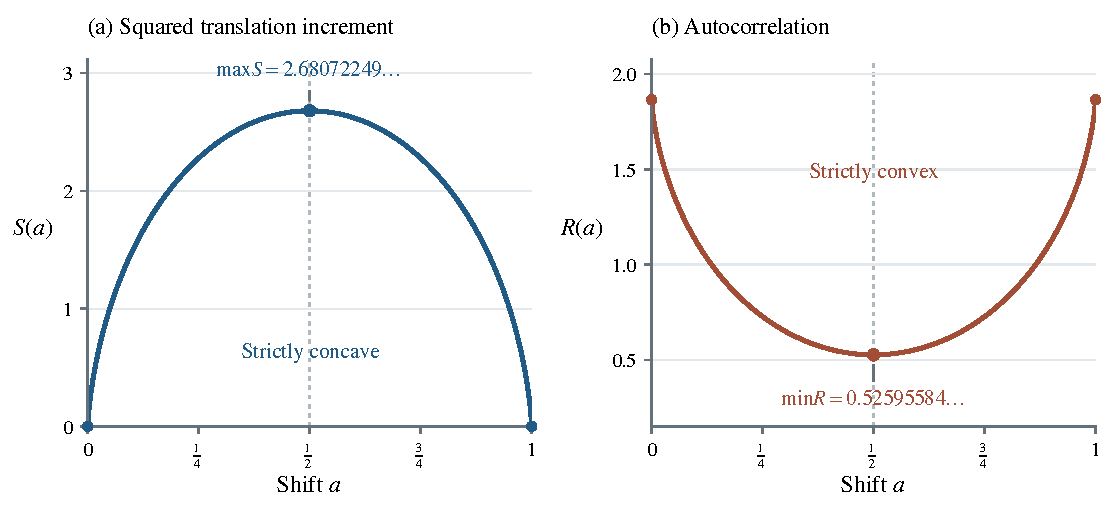
\includegraphics[width=\textwidth]{figures/gamma_correlation_figure.pdf}
\caption{Periodic log-Gamma correlations. The squared translation increment
$S(a)$ is strictly concave, and the autocorrelation $R(a)=R(0)-S(a)/2$
is strictly convex. The dashed guides mark the unique interior extrema at
$a=1/2$. The curves use the convergent series of
Theorem~\ref{gamma:thm:loggamma-concavity} and analytic endpoint limits;
the shape assertions are proved above.}
\label{gamma:fig:correlation}
\end{figure}

\begin{corollary}[Sharp endpoint expansion]
\label{gamma:cor:sharp-cusp}
As $a\downarrow0$,
\begin{align}
 S(a)={}&a\left[\log^2\frac1a+2\log\frac1a+2+\frac{\pi^2}{3}\right]
       +\left(2\gamma_1-\frac{\pi^2}{3}\right)a^2\notag\\
 &-\frac{a^4}{3}\left[\frac32\zeta(3)+\zeta'(3)\right]+O(a^6).
 \label{gamma:eq:sharp-cusp}
\end{align}
The leading behavior is $S(a)\sim a\log^2(1/a)$, with the full
coefficient polynomial and the first analytic corrections explicit.
\end{corollary}

\begin{corollary}[Effective truncation]
\label{gamma:cor:tail}
Let $S_N(a)$ be the right side of
\eqref{gamma:eq:loggamma-increment-series} truncated after $j=N$, where
$N\ge2$. Then
\begin{equation}
 0<S_N(a)-S(a)
 \le\frac{2\zeta(3)[1+\log(2N+2)]}{(N+1)^2}
             \frac{a^{2N+2}}{1-a^2}.
 \label{gamma:eq:tail-bound}
\end{equation}
By symmetry one can always replace $a$ by $\min(a,1-a)\le1/2$ before
evaluating this series.
\end{corollary}

\begin{proof}
The omitted coefficients have one sign. For $j\ge2$,
\[
 0<H_{2j-2}\zeta(2j-1)+\zeta'(2j-1)
    <\zeta(3)[1+\log(2j)],
 \qquad j(2j-1)\ge j^2.
\]
The function $(1+\log(2x))/x^2$ decreases for $x\ge1$.
Majorizing it at $x=N+1$ and summing the geometric tail proves
\eqref{gamma:eq:tail-bound}.
\end{proof}

\subsection{The extremal half-shift and a geometric zeta identity}

\begin{corollary}[Exact maximum]
\label{gamma:cor:half-maximum}
Let $q=\log2$ and $A=\gamma+\log(2\pi)$. Then
\begin{equation}
 \begin{split}
 S(1/2)={}&\frac{3\zeta''(2)+2(q-3A)\zeta'(2)}{2\pi^2}
       +\frac{A^2}{4}-\frac{Aq}{6}-\frac{q^2}{12}+\frac{\pi^2}{16}\\
 ={}&2.68072248798050738482152413952\ldots .
 \end{split}
 \label{gamma:eq:half-maximum}
\end{equation}
Equating this value with the convergent shift expansion gives
\begin{equation}
 \sum_{j=2}^{\infty}\frac{2[H_{2j-2}\zeta(2j-1)+\zeta'(2j-1)]}
                  {4^j j(2j-1)}
 =1+\log2+\frac{\log^2 2}{2}+\frac{\pi^2}{12}
              +\frac{\gamma_1}{2}-S(1/2).
 \label{gamma:eq:dyadic-series}
\end{equation}
\end{corollary}

\begin{proof}
In \eqref{gamma:eq:R-polylog}, use
$\Li_w(-1)=(2^{1-w}-1)\zeta(w)$. Hence
\[
 S(1/2)=\left.\frac1{\pi^2}
   \left[(\partial_w-A)^2+\frac{\pi^2}{4}\right]
       [(2-2^{1-w})\zeta(w)]\right|_{w=2}.
\]
At $w=2$, the three derivatives of $2-2^{1-w}$ required here are
$3/2$, $q/2$, and $-q^2/2$. Expanding and using $\zeta(2)=\pi^2/6$
proves \eqref{gamma:eq:half-maximum}. Substitution of $a=1/2$ into
\eqref{gamma:eq:loggamma-increment-series} proves
\eqref{gamma:eq:dyadic-series}.
\end{proof}

\section{Balanced negative polygamma correlations}
\label{gamma:sec:negative-polygamma}

For an integer $m\ge1$, define the classical balanced normalization
\begin{equation}
 \Psi_m(x)=\frac{\zeta'(1-m,x)+H_{m-1}\zeta(1-m,x)}{(m-1)!}.
 \label{gamma:eq:balanced}
\end{equation}
This is the Espinosa--Moll balanced negapolygamma
\cite{gamma:EspinosaMoll2004}. In particular
$\Psi_1=J_1=g-\ell/2$. It differs from the zero-based repeated
integrals of $g$ used elsewhere in the manuscript by explicit
polynomials. The normalization must be specified before periodizing:
polynomial changes can change endpoint jumps and Fourier decay.

For $m\ge2$, $\Psi_m'=\Psi_{m-1}$,
$\int_0^1\Psi_m=0$, and the endpoint values match.
The same mean-zero assertion holds for $m=1$, whose left endpoint is
logarithmically singular. These facts follow directly from the Hurwitz
shift and derivative identities.

\begin{theorem}[One polylogarithmic operator for the integrated tower]
\label{gamma:thm:balanced-correlation}
For all integers $m,n\ge1$ and $0<a<1$,
\begin{equation}
 \begin{split}
 &\int_0^1\Psi_m(x)\Psi_n(\{x+a\})\,dx\\
 &\quad=\frac2{(2\pi)^{m+n}}
 \Re\left[
    e^{\pi i(m-n)/2}
    \left((\partial_w-A)^2+\frac{\pi^2}{4}\right)
    \Li_w(e^{2\pi ia})\right]_{w=m+n},
 \qquad A=\gamma+\log(2\pi).
 \end{split}
 \label{gamma:eq:balanced-correlation}
\end{equation}
The zero-shift value is obtained by replacing $\Li_w$ with $\zeta(w)$.
At every rational shift, all terms reduce by a finite Fourier transform
to Hurwitz zeta values and their first two spectral derivatives at the
positive integer $m+n$.
\end{theorem}

\begin{proof}
Differentiate \eqref{gamma:eq:hurwitz-fourier} at $s=1-m$ and add the
$H_{m-1}$ multiple. Since
$\psi(m)=H_{m-1}-\gamma$, the harmonic numbers cancel, giving
\begin{equation}
 \widehat\Psi_m(k)
 =\frac{\gamma+\log(2\pi ik)}{(2\pi ik)^m},
 \qquad k\ne0;\qquad \widehat\Psi_m(0)=0.
 \label{gamma:eq:balanced-fourier}
\end{equation}
For $m=1$ this is interpreted in $L^2$; for $m\ge2$ the series is
absolutely convergent. Parseval's product formula therefore applies
in every case. For $k>0$, the product of the opposite-index
coefficients has modulus factor
$(A+\log k)^2+\pi^2/4$ and phase $e^{\pi i(n-m)/2}$.
Combining both signs of $k$ gives
\eqref{gamma:eq:balanced-correlation} because
$\partial_w k^{-w}=-(\log k)k^{-w}$.
The rational-shift statement follows by twice differentiating
\[
 \Li_w(e^{2\pi ip/q})
    =q^{-w}\sum_{r=1}^q e^{2\pi ipr/q}\zeta(w,r/q).
\]
\end{proof}

\begin{corollary}[Exact regularity threshold]
\label{gamma:cor:sobolev}
The periodized function $\Psi_m$ belongs to the circle Sobolev space
$H^\sigma$ exactly when $\sigma<m-1/2$. More generally, for any
$k,r\ge0$, the periodized function
$x\mapsto\partial_s^r\zeta(-k,x)$ belongs to $H^\sigma$ exactly when
$\sigma<k+1/2$.
\end{corollary}

\begin{proof}
With the Fourier definition
$\|f\|_{H^\sigma}^2\asymp\sum_k(1+k^2)^\sigma|\widehat f(k)|^2$,
\eqref{gamma:eq:balanced-fourier} reduces the first claim to convergence
of $\sum_{k\ge2}k^{2\sigma-2m}\log^2k$.
For a general spectral jet, differentiating
\eqref{gamma:eq:hurwitz-fourier} gives
\[
 |\widehat{\partial_s^r\zeta(-k,\cdot)}(n)|
 \sim\frac{k!}{(2\pi)^{k+1}}
              \frac{(\log n)^r}{n^{k+1}}\qquad(n\to+\infty),
\]
with the same power law at negative frequencies.
The comparison series converges exactly below the stated threshold,
including divergence at equality.
\end{proof}

\begin{remark}[Boundary of ordinary integral formulas]
\label{gamma:rem:boundary}
The restriction $m,n\ge1$ in
Theorem~\ref{gamma:thm:balanced-correlation} is essential. The next
derivative is the ordinary digamma function, with a $1/x$ singularity;
periodic shifted products containing it need an explicitly prescribed
finite-part or distributional interpretation. The absolutely
convergent integral theorem does not silently provide such a
regularization.
\end{remark}
